% Figura 2: Trajetória Evolutiva — Gráfico simplificado, cabe na margem ABNT
\begin{figure}[H]
\centering
\resizebox{\textwidth}{!}{%
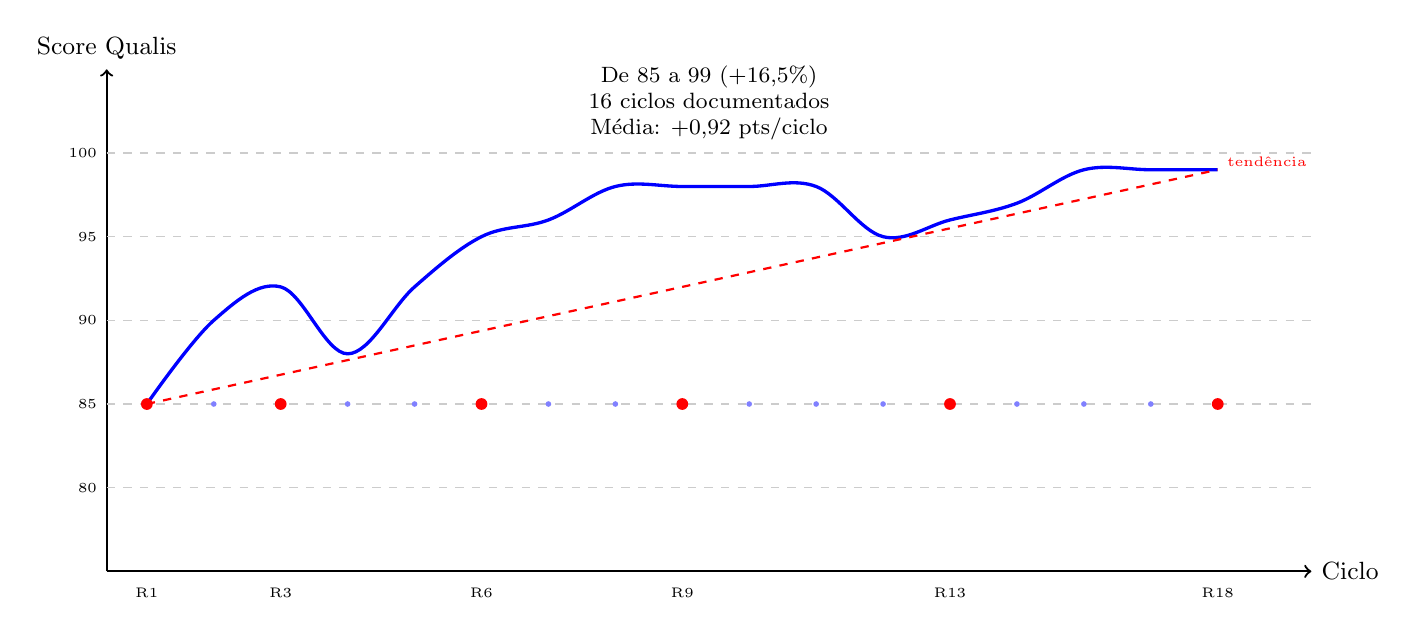
\begin{tikzpicture}[scale=0.85]
% Eixos
\draw[->, thick] (0,0) -- (18,0) node[right] {\small Ciclo};
\draw[->, thick] (0,0) -- (0,7.5) node[above] {\small Score Qualis};

% Grade Y
\foreach \y in {80,85,90,95,100} {
    \draw[dashed, gray!40] (0,{(\y-75)/4}) -- (18,{(\y-75)/4});
    \node[left, font=\tiny] at (0,{(\y-75)/4}) {\y};
}

% Linha de evolução
\draw[blue, very thick] plot[smooth, tension=0.6] coordinates {
    (0.6, {10/4})    % R1: 85
    (1.6, {15/4})    % R2: 90
    (2.6, {17/4})    % R3: 92
    (3.6, {13/4})    % R4: 88
    (4.6, {17/4})    % R5: 92
    (5.6, {20/4})    % R6: 95
    (6.6, {21/4})    % R7: 96
    (7.6, {23/4})    % R8: 98
    (8.6, {23/4})    % R9: 98
    (9.6, {23/4})    % R10: 98
    (10.6, {23/4})   % R11: 98
    (11.6, {20/4})   % R12: 95
    (12.6, {21/4})   % R13: 96
    (13.6, {22/4})   % R14: 97
    (14.6, {24/4})   % R15: 99
    (15.6, {24/4})   % R16: 99
    (16.6, {24/4})   % R17-18: 99
};

% Marcadores principais (apenas alguns para clareza)
\foreach \x/\lab in {0.6/R1,2.6/R3,5.6/R6,8.6/R9,12.6/R13,16.6/R18} {
    \fill[red] (\x,{10/4}) circle (2.5pt);
    \node[below, font=\tiny] at (\x,-0.1) {\lab};
}

% Outros marcadores pequenos
\foreach \x in {1.6,3.6,4.6,6.6,7.6,9.6,10.6,11.6,13.6,14.6,15.6} {
    \fill[blue!50] (\x,{10/4}) circle (1.2pt);
}

% Destaque texto
\node[font=\footnotesize, align=center] at (9,7) {De 85 a 99 (+16,5\%)\\16 ciclos documentados\\M\'edia: +0,92 pts/ciclo};

% Linha de tendência tracejada
\draw[red, dashed, thick] (0.6,{10/4}) -- (16.6,{24/4});
\node[font=\tiny, red, right] at (16.6,{24.5/4}) {tend\^encia};
\end{tikzpicture}%
}
\caption{Trajet\'oria evolutiva do ecossistema OpenCode (R1--R18). O score Qualis progrediu de 85/100 para 99/100 (+16,5\%), com taxa m\'edia de melhoria de 0,92 pontos por ciclo. A linha tracejada vermelha indica a tend\^encia linear de melhoria cont\'inua.}
\label{fig:evolucao}
\end{figure}
